\documentclass{beamer}

\mode<presentation> {
\usecolortheme{seagull}

\setbeamertemplate{footline}[page number]}
\usepackage{graphicx} 
\usepackage{booktabs} 
\usepackage{url}
\usepackage{hyperref}
\usepackage{listings}

\AtBeginSection[]{
  \begin{frame}
  \vfill
  \centering
    \usebeamerfont{title}\Huge{\insertsectionhead\par}
  \vfill
  \end{frame}
}

%-------------------------------------------------------------------------

\title[TLKDCC Debugging]{Debugging}
\author{Hans Holmberg}
\institute[LKTP]
{
Linux Kernel Teaching Project \\ 
\medskip
\textit{hans.holmberg@gmail.com}
}
\date{\today}
%------------------------------------------------------------------------
\begin{document}

\begin{frame}
\titlepage

\includegraphics{../common/tux} 
\end{frame}

\begin{frame}
\frametitle{Overview}
\tableofcontents 
\end{frame}

%-----------------------------------------------------------------------
\section{Debug prints}

\begin{frame}
\frametitle{Debug prints in the kernel}
\begin{itemize}
	\item Prints are easy to implement, but comes at a cost
	\item Code size and execution time is affected
	\item Consider what is *really* needed to leave in your code
	\item Don't use printk, use standardized formatting instead:
	\begin{itemize}
		\item \textbf{dev\_warn, dev\_err, .. :} with device pointer
		\item \textbf{pr\_warn, pr\_err, .. :} no device pointer
	\end{itemize}
\end{itemize}
\end{frame}

\begin{frame}[fragile]
\frametitle{Example 1}
\begin{verbatim}
static int __init my_init(void)
{
  if (bus_register(&some_bus)) {
    pr_err("my_module: Failed to register\n");
    goto fail_bus_register;
  }
  pr_info("my_module: init done\n");
  return 0;

fail_bus_register:
  return -1;
}
module_init(my_init);
\end{verbatim}
\end{frame}

\begin{frame}[fragile]
\frametitle{Example 2}
\begin{verbatim}
ssize_t show_attr(struct device *dev,
             struct device_attribute *attr,
             char *buf)
{
  struct my_dev *mdev = to_mdev(dev);
  
  dev_info(dev, "Showing attribute %s\n",
           attr->attr.name);
  
  if (!mdev->handle) {
    dev_err(dev, "Invalid handle\n");
    return 0;
  }
  ...
}
\end{verbatim}
\end{frame}

\begin{frame}
\frametitle{Warning levels}

\begin{table}[h!]
  \begin{tabular}{l l l}
   \toprule
	Level & Meaning & Macros \\
   \midrule
	0 & emergency message & *\_emerg \\
	1 & alert & *\_alert \\
	2 & critical condition & *\_crit \\
	3 & error & *\_err \\
	4 & warning & *\_warn \\
	5 & notice & *\_notice \\
	6 & information & *\_info \\
	7 & debug & *\_debug \\
   \bottomrule
  \end{tabular}
\end{table}

\end{frame}

\begin{frame}
\frametitle{Looking at the logs}
\begin{itemize}
	\item A subset of logs are printed on the serial debug port. To determine the subset, set the kernel commandline parameter loglevel=N, where:
	\begin{itemize}	
		\item \textbf{N = 0 :} nothing is printed
		\item \textbf{N = 8 :} everything is printed
	\end{itemize}
	\item To change log level at runtime:
	\begin{itemize}
		\item	echo  \textless level\textgreater \space \textgreater \space /proc/sys/kernel/printk
	\end{itemize}
	\item To view the logs after boot, use dmesg.
	\begin{itemize}
		\item dmesg -l \textless level\textgreater \space filters messages
	\end{itemize}
\end{itemize}

\end{frame}

\begin{frame}[fragile]
\frametitle{Enabling debug prints compile time}
\begin{itemize}
	\item pr\_debug and dev\_debug are normally empty macros
	\item To enable debugging output, build the appropriate file with -DDEBUG by adding the following line to the Makefile:
	\begin{verbatim}
	FLAGS_[filename].o := -DDEBUG
	\end{verbatim}
\end{itemize}
\end{frame}

\begin{frame}
\frametitle{Dynamic debug}
\begin{itemize}
	\item Dynamic debug is designed to allow you to dynamically enable/disable kernel code to obtain additional kernel information.
	\item If the config option CONFIG\_DYNAMIC\_DEBUG is set, *\_debug calls can be dynamically enabled via debugfs/dynamic\_debug/control
	\item Debug messages can be enabled per:
	\begin{itemize}
		\item source filename
		\item function name
		\item line number ..
	\end{itemize}
	\item See the kernel documentation\footnote{Dynamic debug howto \url{https://www.kernel.org/doc/Documentation/dynamic-debug-howto.txt} \\} for more info.
\end{itemize}
\end{frame}

%-----------------------------------------------------------------------
\section{Tracing}

\begin{frame}
\frametitle{Strace}
\begin{itemize}
	\item A command line tool that intercepts and records the system calls which are called by a process and the signals which are received by a process.
	\item Useful for bug isolation, sanity checking of the kernel ABI and
a great way of learning about kernel/userspace interaction.
	\item Enables debugging of a program without a recompile (or even access to the source code)
\end{itemize}
\end{frame}

\begin{frame}
\frametitle{Ftrace}
\begin{itemize}
	\item A tracer designed to help out developers and
designers of systems to find what is going on inside the kernel.
	\item Very often enabled on production kernels - you can debug your customer's running kernel image.
	\item Minimal overhead
	\item Uses a ring buffer for storing trace data
	\item Versatile - function tracing, event tracing, fast prints...
	\item Great for studing kernel internals
\end{itemize}
\end{frame}

\begin{frame}
\frametitle{Menuconfig - Kernelhacking - Tracers}
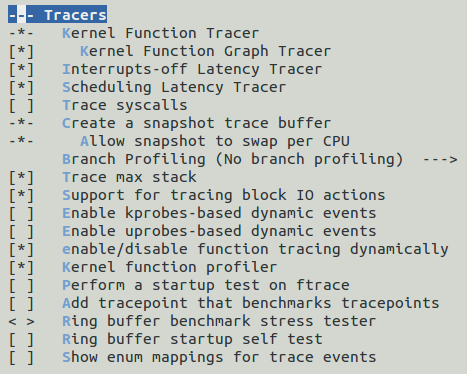
\includegraphics[width=0.7\textwidth]{media/tracingmenuconfig.png}
\end{frame}

\begin{frame}[fragile]
\frametitle{Check available tracers}
\begin{verbatim}
	cd /sys/kernel/debug/tracing
	cat available_tracers
\end{verbatim}
\end{frame}

\begin{frame}
\frametitle{Function trace}
\begin{itemize}
	\item Uses the -pg option in gcc to insert a call to the special function mcount\(\) at the start of every function
	\item During compilation, all calls to mcount is recorded and stored in the kernel
	\item During boot, these are converted to NOP-instructions during to cut away overhead
	\item The NOP's are converted to trace calls when tracing is enabled
	\item The magic is well described in Steven Roestedt's presentation from Linux Plumbers 2014. \footnote{Ftrace Kernel Hooks: More than just tracing \url{https://linuxplumbersconf.org/2014/ocw/system/presentations/1773/original/ftrace-kernel-hooks-2014.pdf} \\}
\end{itemize}
\end{frame}

\begin{frame}[fragile]
\frametitle{Function trace - Example 1}
\begin{verbatim}
	cd /sys/kernel/debug/tracing
	echo function > current_tracer
	echo 1 > tracing_on && sleep 1 && echo 0 > tracing_on
	cat trace
\end{verbatim}
\end{frame}

\begin{frame}[fragile]
\frametitle{Function trace - Example 2}
\begin{verbatim}
	cd /sys/kernel/debug/tracing
	echo pl011* > set_ftrace_filter
	echo function > current_tracer
	cat trace
	echo 1 > tracing_on && sleep 1 && echo 0 > tracing_on
	cat trace
	echo function_graph > current_tracer
	echo 1 > tracing_on && sleep 1 && echo 0 > tracing_on
	cat trace
\end{verbatim}
\end{frame}

\begin{frame}
\frametitle{Trace points}
\begin{itemize}
\item One of the most common uses of ftrace is the event tracing.
Through out the kernel is hundreds of static event points that
can be enabled via the debugfs file system to see what is
going on in certain parts of the kernel.
\item Available events: cat /sys/kernel/debug/tracing/available\_events 
\end{itemize}
\end{frame}

\begin{frame}[fragile]
\frametitle{Trace points example}
What is the irq number for the pl011 interrupt?
\begin{verbatim}
echo irq_handler_entry >> set_event
echo irq_handler_exit >> set_event
echo nop > current_tracer
echo 1 > tracing_on && sleep 1 && echo 0 > tracing_on
cat trace |grep pl011
\end{verbatim}
\end{frame}

\begin{frame}
\frametitle{Trace\_printk}
\begin{itemize}
	\item Printk is great, but has significant overhead and can bog down the system and change timing.
	\item trace\_printk has minimal overhead and writes to the trace buffer instead of of the console. It can be used in any context.
	\item printk has an overhead in the order of milliseconds, trace\_printk in microseconds
	\item trace prints will be displayed in all tracer outputs
\end{itemize}
\end{frame}

\begin{frame}[fragile]
\frametitle{Example - Traceprintk}
\tiny
\begin{verbatim}
static irqreturn_t pl011_int (int irq , void * dev_id )
{
   ...
   status = readl ( uap - > port . membase + UART011_MIS );
   trace_printk (" status %#x\n", status );
   ...
\end{verbatim}
\noindent\rule[0.5ex]{\linewidth}{1pt}
\begin{verbatim}
cat/sys/kernel/debug/tracing/trace
#                       _ -----= > irqs-off
#                      /  _----= > need-resched
#                      | /_---= > hardirq / softirq
#                      ||/_--= > preempt - depth
#                      |||/ delay
#       TASK-PID  CPU# ||||      TIMESTAMP FUNCTION
#          | | |   |   || |          |         |
kworker /0:1-549 [000] d.h2     47.102049: pl011_int : status 0 x20
sh -666          [000] d.h2     47.102438: pl011_int : status 0 x20
\end{verbatim}
\end{frame}

\begin{frame}
\frametitle{Other functions}
Ftrace is really powerful and has lots of other uses.\\
Additional tracers: \\
\begin{itemize}
	\item irqsoff : measure max interrupt latency
	\item wakeup : measure max task wakeup latency
\end{itemize}
You can also dynamically trigger tracing, monitor stack usage, and many other things. See the kernel documentation \footnote{Ftrace \url{https://www.kernel.org/doc/Documentation/trace/ftrace.txt}}. \\
Rabin Vincent's presentation from LLC 2013 is also a good source of ftrace tricks and hacks \footnote{Introduction to ftrace \url{http://goo.gl/NttCcp} \\}.
\end{frame}
%-----------------------------------------------------------------------
\section{Crash log analysis}
\begin{frame}
\frametitle{Oops and kernel panics}
\begin{itemize}
	\item \textbf{Panic} : Unrecoverable errors
	\item \textbf{Oops} : Non-fatal error, kernel continues (but might not work correctly)
\end{itemize}
\end{frame}

\begin{frame}[fragile]
\frametitle{Oops example}
\tiny
\begin{verbatim}
[   41.596330] ------------[ cut here ]------------
[   41.603095] kernel BUG at drivers/input/keyboard/gpio_led_key.c:52!
[   41.611584] Internal error: Oops - BUG: 0 [#1] SMP ARM
[   41.618969] Modules linked in:
[   41.624291] CPU: 2 PID: 91 Comm: irq/184-soc:led Not tainted 4.9.0-rc3-v7+ #4
[   41.633877] Hardware name: BCM2709
[   41.639723] task: b9100000 task.stack: b9108000
[   41.646723] PC is at led_gpio_key_isr+0xc4/0xe0
[   41.653702] LR is at regulator_enable+0xa8/0x14c
[   41.660736] pc : [<80583cb8>]    lr : [<804a3f24>]    psr: 60000013
[   41.660736] sp : b9109ee0  ip : b9109ec0  fp : b9109f04
[   41.677151] r10: 8016f100  r9 : b9bf8e80  r8 : b9bf8d80
[   41.684878] r7 : 00000000  r6 : b9194c00  r5 : 00000000  r4 : b9bf7e10
[   41.693959] r3 : 80a5f9d0  r2 : 00000000  r1 : 00000000  r0 : 00000000
[   41.703034] Flags: nZCv  IRQs on  FIQs on  Mode SVC_32  ISA ARM  Segment user
[   41.712788] Control: 10c5387d  Table: 391f406a  DAC: 00000055
[   41.721158] Process irq/184-soc:led (pid: 91, stack limit = 0xb9108210)
[   41.730480] Stack: (0xb9109ee0 to 0xb910a000)
[   41.737543] 9ee0: 80583bf4 b9bf8e80 00000000 b9b66b40 00000001 b9b66b40 b9109f24 b9109f08
[   41.751388] 9f00: 8016f12c 80583c00 00000004 b9108000 00000000 b9bf8ea4 b9109f5c b9109f28
[   41.765431] 9f20: 8016f460 8016f10c 00000000 8016f278 00000000 b9bf8ec0 00000000 b9bf8e80
[   41.779664] 9f40: 8016f338 00000000 00000000 00000000 b9109fac b9109f60 8013c710 8016f344
[   41.794046] 9f60: 00000000 00000000 00000000 b9bf8e80 00000000 00000000 b9109f78 b9109f78
[   41.808738] 9f80: 00000000 00000000 b9109f88 b9109f88 b9bf8ec0 8013c628 00000000 00000000
[   41.823806] 9fa0: 00000000 b9109fb0 80107e88 8013c634 00000000 00000000 00000000 00000000
[   41.839158] 9fc0: 00000000 00000000 00000000 00000000 00000000 00000000 00000000 00000000
[   41.854878] 9fe0: 00000000 00000000 00000000 00000000 00000013 00000000 00000000 00000000
[   41.870790] [<80583cb8>] (led_gpio_key_isr) from [<8016f12c>] (irq_thread_fn+0x2c/0x44)
[   41.886655] [<8016f12c>] (irq_thread_fn) from [<8016f460>] (irq_thread+0x128/0x1f8)
[   41.902258] [<8016f460>] (irq_thread) from [<8013c710>] (kthread+0xe8/0x104)
[   41.913375] [<8013c710>] (kthread) from [<80107e88>] (ret_from_fork+0x14/0x2c)
[   41.924627] Code: e2422001 e3520000 e583205c 1affffef (e7f001f2) 
[   41.934698] ---[ end trace c6b22157650fc26a ]---
\end{verbatim}
\end{frame}

\begin{frame}[fragile]
\frametitle{Post mortem analysis}
\begin{itemize}
\item If the kernel panics, a common way of debugging is to save the contents of the system memory and analyze it.
\item The kernel can be configured (CONFIG\_CRASH\_DUMP) to boot into a second kernel at separate location in memory, capable of saving the system memory to disk or send it over the network.
\item See the kdump kernel documentation for how to set this up \footnote{kdump \url{https://www.kernel.org/doc/Documentation/kdump/kdump.txt}}
\item When the capture kernel has booted, the dump is available in /proc/vmcore 
\item Wikipedia also has a good page on this \footnote{Wikipedia kdump \url{https://en.wikipedia.org/wiki/Kdump_(Linux)} \\}
\end{itemize}
\end{frame}

\begin{frame}
\frametitle{Analyzing dumps: crashtool}
\begin{itemize}
	\item Developed by Red Hat
	\item Requires a dump file and a kernel image built with symbols included
	\item Provides an interactive environment similar to gdb
	\item Can display information about tasks, display back traces, display log and trace buffers, inspect memory, and much more
	\item See the excellent documentation for more information \footnote{Crash \url{https://people.redhat.com/anderson/crash_whitepaper} \\}
\end{itemize}
\end{frame}

%-----------------------------------------------------------------------
\section{Interactive debug}
\begin{frame}
\frametitle{Kgdb}
\begin{itemize}
	\item Enables in-kernel debugging directly using a non-usb keyboard and vga text console or remotely using a serial port
	\item Possible to stop the kernel, do single stepping, inspect memory
	\item See the documentation \footnote{Kgdb \url{http://free-electrons.com/kerneldoc/latest/DocBook/kgdb/} \\} for how to set it up.
	\item Can be used with QEMU
\end{itemize}
\end{frame}

\begin{frame}
\frametitle{JTAG debugging}
\begin{itemize}
	\item Enables full debugging of the hardware from another machine via a dongle witout affecting the kernel.
	\item Dongles range from relatively inexpensive to extremely expensive and feature-rich.
	\item GDB can be used as a front-end.
\end{itemize}
\end{frame}

%-----------------------------------------------------------------------
\begin{frame}
\Huge{\centerline{Thanks!}}
\end{frame}

\end{document} 
